\documentclass{beamer}
\usetheme{Antibes}

\usepackage{fontspec}
\usepackage[catalan]{babel}
\usepackage{hyperref}

\AtBeginSection[]
{
	\begin{frame}
		\frametitle{Contingut}
		\tableofcontents[currentsection]
	\end{frame}
}

\AtBeginSubsection[]
{
	\begin{frame}
		\frametitle{Contingut}
		\tableofcontents[currentsection,currentsubsection]
	\end{frame}
}

\title{Construcció d'una orquestra amb Raspberry Pi}
\author{Arnau Canyadell Miquel \and Joan Marcè Igual}

\begin{document}

\frame{\titlepage}
\section{Introducció}

\begin{frame}
	Crear amb Raspberry Pi una orquestra musical formada per un director i uns quants músics que interpreten el que els mana el director.
	\begin{figure}
		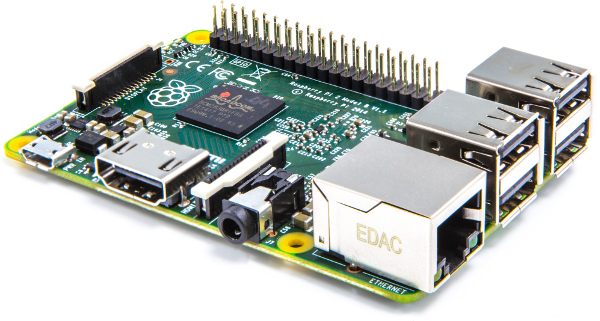
\includegraphics[width=0.475\linewidth]{images/raspberry}
		\hfill
		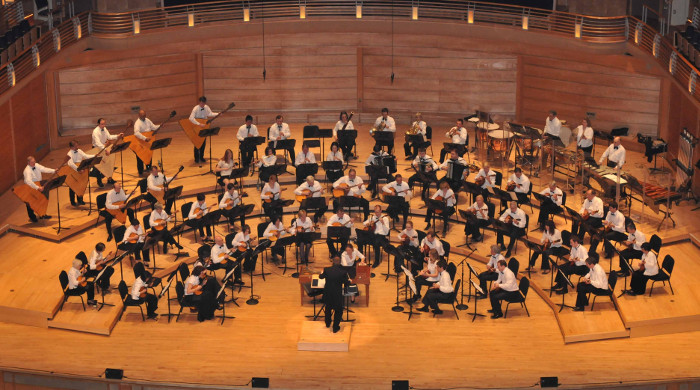
\includegraphics[width=0.475\linewidth]{images/orchestra}
	\end{figure}
\end{frame}

\section{Metodologia}

\begin{frame}
	\begin{itemize}[<+->]
		\item Repositori: \url{https://github.com/jmigual/projecte2}
		\item Trello amb objectius a curt i a llarg termini
		\item Llenguatge de programació: \texttt{Python}
	\end{itemize}
	\begin{figure}
		\hfill
		\includegraphics<1->[width=0.25\textwidth]{images/github}
		\hfill
		\includegraphics<2->[width=0.4\textwidth]{images/trello}
		\hfill
		\includegraphics<3->[width=0.25\textwidth]{images/python}
		\hfill
	\end{figure}
\end{frame}

\section{Feina feta}
\begin{frame}
	\begin{itemize}
		\item Establiment dels objectius
		\item Analitzat el codi del director
		\item Programat una primera versió del client (intèrpret o músic)
	\end{itemize}
\end{frame}

\section{Objectius}
\begin{frame}
	\frametitle{Idees a curt termini}
	\begin{description}
		\item[17 de març] Rebre música d'un ordinador
		\item[24 de març] Enviar música a una Raspberry Pi
		\item[31 de març] Reproduir música
	\end{description}
\end{frame}

\begin{frame}
	\frametitle{Idees a llarg termini}
	\begin{itemize}[<+->]
		\item Bot de Telegram que reprodueixi midi
		\item Enviar música des del mòbil
	\end{itemize}
	\begin{figure}
		\hfill
		\includegraphics<1->[width=0.2\textwidth]{images/telegram}
		\hfill
		\includegraphics<2->[width=0.475\textwidth]{images/mobile}
		\hfill
	\end{figure}
\end{frame}

\section{Material}
\begin{frame}
	Cal una gran quantitat de Raspberry Pi per fer una orquestra el més gran possible. 
	
	Com a mínim seria necessari:
	\begin{itemize}
		\item 1 director
		\item 4 músics
	\end{itemize}
\end{frame}

\end{document}